%======================================================================
%   One-page CV – Template 03  (pdfLaTeX-ready)
%======================================================================
\documentclass[11pt,a4paper]{article}

%---------- Encodage, langue ------------------------------------------
\usepackage[T1]{fontenc}
\usepackage[utf8]{inputenc}
\usepackage[british]{babel}

%---------- Géométrie --------------------------------------------------
\usepackage[left=2cm,right=2cm,top=2.2cm,bottom=2.2cm]{geometry}
\setlength{\parindent}{0pt}
\setlength{\parskip}{0pt}
\usepackage{setspace}
\setstretch{1.15}

%---------- Police & microtypographie ----------------------------------
\IfFileExists{FiraSans.sty}
  {\usepackage[sfdefault]{FiraSans}}
  {\renewcommand\familydefault{\sfdefault}}

\usepackage[stretch=25,shrink=25,tracking=true]{microtype}

%---------- Icônes & couleurs ------------------------------------------
\usepackage{fontawesome5}
\usepackage{xcolor}
\definecolor{accent}{HTML}{161616}

%---------- Commandes pratiques ----------------------------------------
\newcommand{\headline}[1]{\textsc{\large #1}}

\newcommand{\sectiontitle}[1]{%
  \vspace{1em}\textbf{\uppercase{#1}}\par\vspace{.2em}
  \hrule height 0.7pt\relax\vspace{.8em}}

\newcommand{\job}[4]{% titre, entreprise, dates, bullets
  \textbf{#1} \hfill \faBuilding\;#2 \hfill \faCalendar\;#3\par
  \begin{itemize}\setlength\itemsep{.2em}#4\end{itemize}\vspace{.6em}}

\newcommand{\edu}[3]{% diplôme, établissement, dates
  \textbf{#1}\par
  {\small #2}\hfill\faCalendar\;#3\par\vspace{.8em}}

%======================================================================
\begin{document}\small

%------------------- En-tête : nom & tagline ---------------------------
\begin{center}
  {\Huge\bfseries Pape Saliou FALL}\par
  \vspace{.3em}
  \headline{DATA SCIENTIST}\par
  \vspace{.8em}
  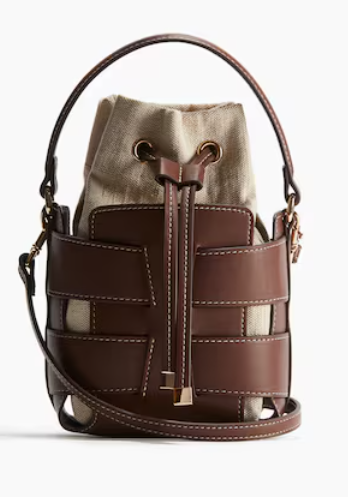
\includegraphics[width=3cm,height=3cm,clip,keepaspectratio]{90575f3fb48947dfaf496b4c9bac508a.png}
\end{center}\vspace{1em}

%------------------- Coordonnées --------------------------------------
\begin{tabular*}{\textwidth}{@{\extracolsep{\fill}}lll}
\faEnvelope[regular]\; papesalioufall2@gmail.com &
\faPhone\; 07\,53\,48\,14\,53 &
\faMapMarker*\; 15 Rue des Écoles, 75005 Paris, France
\end{tabular*}

%------------------- Profil -------------------------------------------
\vspace{1.2em}
\fboxsep=8pt
\colorbox{gray!8}{%
  \parbox{\dimexpr\linewidth-2\fboxsep}{%
  \small Data Scientist doté d’une double compétence en mathématiques appliquées et en data science, diplômé de Sorbonne Université. Plus de 1 an d’expérience dans le développement de modèles prédictifs, l’automatisation de pipelines de données et la création de tableaux de bord décisionnels. Solide maîtrise de Python, SQL et des techniques de machine-learning avancées, avec un goût prononcé pour la résolution de problématiques métier complexes et la vulgarisation des insights auprès des parties prenantes.}}

%======================================================================
\sectiontitle{Experience}

\job
  {Data Scientist}
  {Prepaya}
  {Sept.~2022 – Aug.~2023}
  {
    \item Conçu et déployé des modèles de prédiction du \emph{churn} réduisant le taux d’attrition de 18\,\%.
    \item Automatisé le pipeline de collecte et de nettoyage des données avec Python et Airflow, diminuant le temps de préparation de 40\,\%.
    \item Implémenté un tableau de bord interactif sous Power~BI pour le suivi en temps réel des KPI business.
    \item Collaboré avec les équipes Produit et Marketing afin de transformer les insights data en recommandations actionnables.
  }

%======================================================================
\begin{minipage}[t]{0.47\textwidth}
%===================== COMPÉTENCES ====================================
\sectiontitle{Skills}

\textbf{Programming \& Analytics}\par
Python, R, SQL, Machine Learning, Deep Learning (TensorFlow, PyTorch), Natural Language Processing, Time-Series Forecasting, Statistics \& Probability.

\vspace{.6em}
\textbf{Data Engineering}\par
Data Cleaning \& Feature Engineering, Big Data (Spark, Hadoop), Cloud Computing (AWS, GCP), Docker, Git.

\vspace{.6em}
\textbf{Visualisation \& BI}\par
Tableau, Power~BI, Matplotlib, Seaborn.

\vspace{.6em}
\textbf{Languages}\par
Français (natif), Anglais (courant)

\vspace{.6em}
\textbf{Hobbies}\par
Football, échecs, photographie urbaine
\end{minipage}
\hfill
\begin{minipage}[t]{0.47\textwidth}
%===================== ÉDUCATION ======================================
\sectiontitle{Education}

\edu{Master~2\,–\,Data Science}
    {Sorbonne Université}
    {2022–2023}

\edu{Licence\,–\,Mathématiques Appliquées}
    {Université Cheikh Anta Diop, Dakar}
    {2018–2021}

%===================== CERTIFICATIONS =================================
\sectiontitle{Certifications}

\textbf{TensorFlow Developer Certificate}\par
{\small Google}\hfill\faCalendar\;2024-02\par\vspace{.6em}

\textbf{IBM Data Science Professional Certificate}\par
{\small Coursera}\hfill\faCalendar\;2023-06\par

\end{minipage}

\end{document}